\usetikzlibrary{patterns, intersections, math}

% use the 7-class colorbrewer "setdark2" palette (skipping color 6 because it's too light)
\definecolor{g1}{HTML}{1b9e77}
\definecolor{g2}{HTML}{d95f02}
\definecolor{g1s1}{HTML}{7570b3}
\definecolor{g1s2}{HTML}{e7298a}
\definecolor{g2s1}{HTML}{66a61e}
\definecolor{g1s3}{HTML}{a6761d}

% pseudotaxa are all gray
\definecolor{g1s4}{HTML}{bbbbbb}
\definecolor{g2s2}{HTML}{bbbbbb}
\definecolor{g3}{HTML}{bbbbbb}
\definecolor{g3s1}{HTML}{bbbbbb}
\definecolor{g3s2}{HTML}{bbbbbb}

\definecolor{unknown}{HTML}{aaaaaa}

%define the family clustering radius
\def\famrad{35}
% define the genus clustering radius
\def\genrad{23}
% define the species clustering radius in genus g1
\def\spradA{13}
% define the species clustering radius in genus g2
\def\spradB{8}

% define the radius of an ASV symbol
\def\asvrad{1.5}

\def\known{known}
\def\denovo{denovo}
\def\reffirst{ref1}
\def\refsecond{ref2}

% define ASVs
% each entry is x/y/genus/species/radius/type
\newcommand{\asvs}{%
  38.181816/215.75/g1/g1s1/\spradA/known,%
%  33.409092/217.22728/g1/g1s1/\spradA/known,%
%  37.613636/219.61363/g1/g1s1/\spradA/known,%
%  16.136364/230.97728/g1/g1s1/\spradA/known,%
  15.681818/237.56818/g1/g1s1/\spradA/known,%
  23.977272/245.63637/g1/g1s1/\spradA/ref1,%
  30.795454/227/g1/g1s1/\spradA/ref1,%
  15.113636/266.54544/g1/g1s2/\spradA/known,%
%  15.681818/269.15909/g1/g1s2/\spradA/known,%
  23.977272/267.22726/g1/g1s3/\spradA/known,%
  96/243/g2/g2s1/\spradB/ref1,%
  98.75/210.29544/g2/g2s2/\spradB/denovo,%
  120/207.11363/g2/g2s1/\spradB/known,%
  %118.181816/210.97728/g2/g2s1/\spradB/known,%
  121.13636/219.04546/g2/g2s1/\spradB/known,%
  99/232/g2/g2s1/\spradB/known,%
  103/255/g2/g2s1/\spradB/ref2,%
  56.704544/278.59091/g1/g1s4/\spradA/denovo,%
  58/289.11365/g1/g1s4/\spradA/denovo,%
  45.56818/285.29544/g1/g1s4/\spradA/denovo,%
  30.136364/296.84091/g1/g1s4/\spradA/denovo,%
  70.11364/295.06818/g1/g1s4/\spradA/denovo,%
  145/290/g3/g3s1/\spradB/denovo,%
  155/290/g3/g3s1/\spradB/denovo,%
  120/304/g3/g3s2/\spradB/denovo,%
  132/306/g3/g3s2/\spradB/denovo,%
  151/282/g3/g3s1/\spradB/denovo%
}

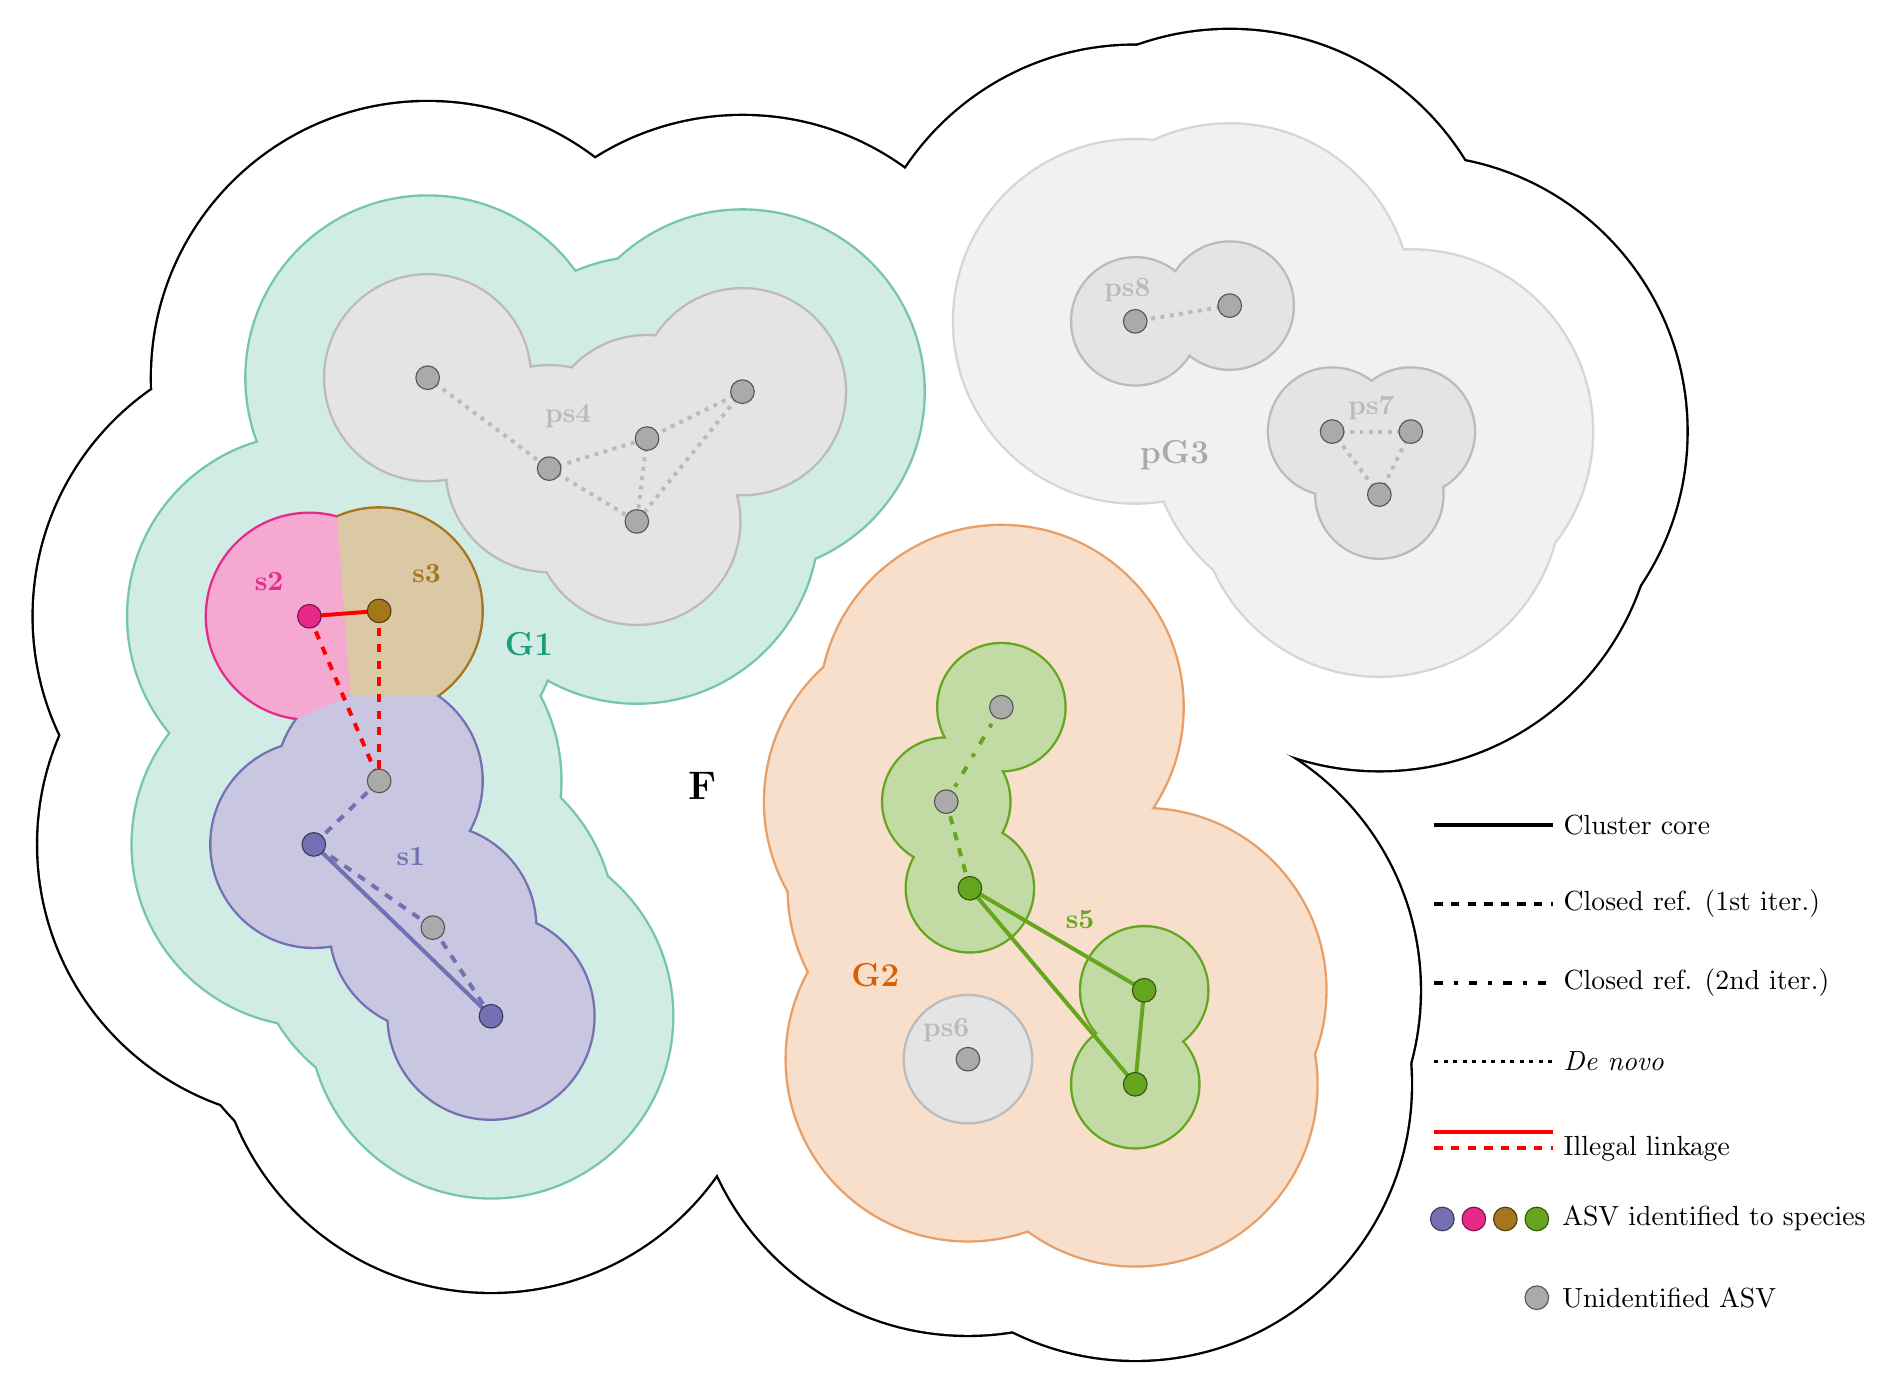
\begin{tikzpicture}[x=1mm, y=1mm]

% define styles for objects
% ASVs are represented as small circles
% the fill color will be defined separately each time it is used, and the
% outline will always be a darker version of the same color
\tikzstyle{asv}=[circle, draw=black!50, fill=black!50, inner sep=0pt]

% define the genus of each asv in a list
\def\asvgenus{
  g1, g1, g1, g1, g1, g1, g1, g1, g1, g1,
  g2, g2, g2, g2, g2, g2, g2, g1, g1, g1,
  g1, g1, g2
}

% define the known species of each asv in a list
\def\asvknown{
  g1s1, g1s1, g1s1, g1s1, g1s1, unknown, unknown, g1s2, g1s2, g1s2,
  unknown, unknown, g2s1, g2s1, g2s1, unknown, unknown, unknown, unknown, unknown,
  unknown, unknown, unknown
}

% draw family cluster as dashed outline
\foreach \x / \y in \asvs {
  \draw[line width=0.6mm] (\x, \y) circle (\famrad);
}

% clear interior of family cluster
\foreach \x / \y in \asvs {
  \fill[white] (\x, \y) circle (\famrad);
}

% draw genus cluster outlines with thicker lines
\foreach \x / \y / \color in \asvs {
  \draw[color=\color!60, line width=0.6mm] (\x, \y) circle (\genrad);
}

%shade genus clusters with a very light version of the color
\foreach \x / \y / \color in \asvs {
  \fill[color=\color!20] (\x, \y) circle (\genrad);
}

% draw species cluster outlines with thinner lines
\foreach \x / \y / \genus / \species / \radius [count = \i] in \asvs {
  \begin{scope}
    \path[name path=self, save path=\self] (\x, \y) circle (\radius);
    \foreach \xb / \yb / \genusb / \speciesb / \radiusb [count = \j] in \asvs {
      \ifnum\i>\j
        %check if the two circles are the same species
        \ifx\species\speciesb
        \else
        %\pgfmathsetmacro{\dist}{sqrt((\x - \xb)^2 + (\y - \yb)^2)}
        %\ifdim\dist pt<2*\radius pt
        \path[name path=other] (\xb, \yb) circle (\radiusb);
          \clip [name intersections={of = self and other, name = i, total=\t}]
            \ifnum\t>1
              (i-1) -- (i-2) -- ([turn] 0:\radiusb) -- ([turn] 90:2*\radiusb) -- ([turn] 90:4*\radiusb) -- ([turn] 90:2*\radiusb) --cycle;


            \fi;
        \fi
      \fi
    }
      \draw[\species, line width=0.6mm] (\x, \y) circle (\radius);
  \end{scope}}

% shade species clusters with a light version of the color
% when there are two species within the same radius of each other, we need to
% calculate the line between them and set a clip path to avoid shading the
% entire circle
\foreach \x / \y / \genus / \species / \radius [count = \i] in \asvs {
  \pgfinterruptboundingbox
  \begin{scope}
    \path[name path=self, save path=\self] (\x, \y) circle (\radius);
    \foreach \xb / \yb / \genusb / \speciesb / \radiusb [count = \j] in \asvs {
      \ifnum\i>\j
        %check if the two circles are the same species
        \ifx\species\speciesb
        \else
        %\pgfmathsetmacro{\dist}{sqrt((\x - \xb)^2 + (\y - \yb)^2)}
        %\ifdim\dist pt<2*\radius pt
        \path[name path=other] (\xb, \yb) circle (\radiusb);
          \clip [name intersections={of = self and other, name = i, total=\t}]
            \ifnum\t>1
              (i-1) -- (i-2) -- ([turn] 0:\radiusb) -- ([turn] 90:2*\radiusb) -- ([turn] 90:4*\radiusb) -- ([turn] 90:2*\radiusb) --cycle;


            \fi;
        \fi
      \fi
    }
      \fill[\species!40] (\x, \y) circle (\radius);
  \end{scope}
  \endpgfinterruptboundingbox
}

% draw linkage between ASVs
\foreach \x / \y / \genus / \species / \radius / \type [count = \i] in \asvs {
  \begin{scope}
    \foreach \xb / \yb / \genusb / \speciesb / \radiusb / \typeb [count = \j] in \asvs {
      \ifnum\i>\j
        %check the distance between the ASVs
        \pgfmathparse{notgreater(veclen(\x - \xb, \y - \yb), \radius + \radiusb)}
        \ifnum\pgfmathresult=1
          \ifx\species\speciesb
            \ifx\type\denovo
              \draw[\species, line width=0.5mm, dotted] (\x, \y) -- (\xb, \yb);
            \else
              \ifx\type\known
                \ifx\typeb\known
                  \draw[\species, line width=0.5mm] (\x, \y) -- (\xb, \yb);
                \else
                  \draw[\species, line width=0.5mm, dashed] (\x, \y) -- (\xb, \yb);
                \fi
              \else
                \ifx\typeb\known
                  \draw[\species, line width=0.5mm, dashed] (\x, \y) -- (\xb, \yb);
                \else
                  \ifx\type\refsecond
                    \ifx\typeb\reffirst
                      \draw[\species, line width=0.5mm, loosely dash dot] (\x, \y) -- (\xb, \yb);
                    \fi
                  \else
                    \ifx\type\reffirst
                      \ifx\typeb\refsecond
                        \draw[\species, line width=0.5mm, loosely dash dot] (\x, \y) -- (\xb, \yb);
                      \fi
                    \fi
                  \fi
                \fi
              \fi
            \fi
          \else
            \ifx\type\known
              \ifx\typeb\known
                \draw[red, line width=0.5mm] (\x, \y) -- (\xb, \yb);
              \else
                \draw[red, line width=0.5mm, dashed] (\x, \y) -- (\xb, \yb);
              \fi
            \else
              \draw[red, line width=0.5mm, dashed] (\x, \y) -- (\xb, \yb);
            \fi
          \fi
        \else
          \ifx\species\speciesb
            \ifx\type\known
              \ifx\typeb\known
                \draw[\species, line width=0.5mm] (\x, \y) -- (\xb, \yb);
              \fi
            \fi
          \fi
        \fi
      \fi
    }
  \end{scope}
}

% shade de-novo clustered ASVs using a very light grey with a dotted pattern
%\foreach \x / \y / \genus / \species / \radius / \type in \asvs {
%  \ifx\type\denovo
%    \fill[pattern=dots, pattern color=\species] (\x, \y) circle (\radius);
%  \fi
%}

% shade second.stage reference clustered ASVs using a gray version of their color
%\foreach \x / \y / \genus / \species / \radius / \type in \asvs {
  %\ifx\type\refsecond
%    \fill[pattern=crosshatch, pattern color=\species!80] (\x, \y) circle (\radius);
%  \fi
%}
% shade first.stage reference clustered ASVs using a light version of their color
%\foreach \x / \y / \genus / \species / \radius / \type in \asvs {
%  \ifx\type\reffirst
%    \fill[\species!60] (\x, \y) circle (\radius);
%    \fill[pattern=north east lines, pattern color=\species!80] (\x, \y) circle (\radius);
%  \fi
%}
% shade known clustered ASVs using their color
%\foreach \x / \y / \genus / \species / \radius / \type in \asvs {
%  \ifx\type\known
%    \fill[\species!60] (\x, \y) circle (\radius);
%  \fi
%}

% draw ASV points
\foreach \x / \y / \genus / \species / \radius / \type in \asvs {
  \ifx\type\known
    \draw[\species!50!black, fill=\species] (\x, \y) circle (\asvrad);
  \else
    \draw[unknown!50!black, fill=unknown] (\x, \y) circle (\asvrad);
  \fi
}

% draw family cluster label with big text
\node[align=center,node font=\Large\bfseries] at (65, 245) {F};

% draw genus cluster labels with medium text
\node[align=center,node font=\large\bfseries,color=g1] at (43, 263) {G1};
\node[align=center,node font=\large\bfseries,color=g2] at (87, 221) {G2};
\node[align=center,node font=\large\bfseries,color=unknown] at (125, 287) {pG3};

% draw species cluster labels with small text
\node[align=center,node font=\bfseries,color=g1s1] at (28, 236) {s1};
\node[align=center,node font=\bfseries,color=g1s2] at (10, 271) {s2};
\node[align=center,node font=\bfseries,color=g1s3] at (30, 272) {s3};
\node[align=center,node font=\bfseries,color=g1s4] at (48, 292) {ps4};
\node[align=center,node font=\bfseries,color=g2s1] at (113, 228) {s5};
\node[align=center,node font=\bfseries,color=g2s2] at (96, 214) {ps6};
\node[align=center,node font=\bfseries,color=g3s1] at (150, 293) {ps7};
\node[align=center,node font=\bfseries,color=g3s2] at (119, 308) {ps8};

% draw legend
\draw [line width=0.5mm] (158,240) -- (173,240) node[right] {Cluster core};
\draw [line width=0.5mm, dashed] (158,230) -- (173,230) node[right] {Closed ref. (1st iter.)};
\draw [line width=0.5mm, loosely dash dot] (158,220) -- (173,220) node[right] {Closed ref. (2nd iter.)};
\draw [line width=0.5mm, dotted] (158,210) -- (173,210) node[right] {\emph{De novo}};
\draw [line width=0.5mm, red] (158,201) -- (173,201);
\draw [line width=0.5mm, red, dashed] (158,199) -- (173,199) node[right, color = black] {Illegal linkage};

% color swatches for known species
\draw [g1s1!50!black, fill=g1s1] (159,190) circle (\asvrad);
\draw [g1s2!50!black, fill=g1s2] (163,190) circle (\asvrad);
\draw [g1s3!50!black, fill=g1s3] (167,190) circle (\asvrad);
\draw [g2s1!50!black, fill=g2s1] (171,190) circle (\asvrad) node[right=2mm, color = black] {ASV identified to species};
\draw [unknown!50!black, fill=unknown] (171,180) circle (\asvrad) node[right=2mm, color = black] {Unidentified ASV};


\end{tikzpicture}
